\documentclass[../../main.tex]{subfiles}
\begin{document}

\subsection*{3.5}
Una carica è distribuita all'interno di una superfice cilindrica indefinita con densità $\rho = \rho_0(a-br)$ essendo r la distanza dall'asse e $\rho_0$, a, b costanti.
\\Determinare l'espressione del campo elettrostatico in funzione di r.
\\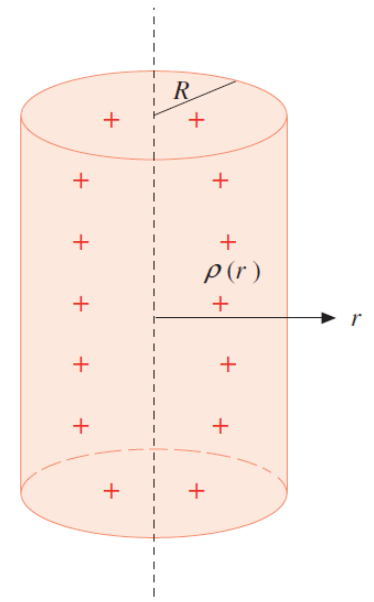
\includegraphics[scale=0.3]{e_3_5.png}
\subsubsection*{Formule utilizzate}
\subsubsection*{Soluzione punto a}
per $0 \le r \le R$
\\$\frac{q(r)}{r} = \lambda (r)$
\\$\lambda(r) = \int_0^r 2r\pi\rho(r) dr= \int_0^r2\pi\rho_0(ar-br^2)dr = 2 \pi\rho_0r^2\left(\frac{a}{2}-\frac{b}{3}r\right)$
\\$E_{int} = \frac{\lambda(r)}{2\pi\epsilon_0r} = \frac{\rho_0r}{2\epsilon_0}\left(a- \frac{2}{3}br\right)$
\\$\lambda(R) = 2\pi\rho_0 R^2\left(\frac{a}{2}-\frac{b}{3}R\right)$
\\$E_{est} = \frac{\lambda(R)}{2pi\epsilon_0r} = \frac{\rho_0R^2}{2\epsilon_0r}\left(a-\frac{2}{3}bR\right)$
\subsubsection*{Soluzione punto b}
\newpage

\end{document}